\documentclass[usenames,dvipsnames]{beamer}


\usetheme{Madrid}
\usecolortheme{dolphin}
\setbeamercolor{title}{fg=NavyBlue}
\setbeamercolor{frametitle}{fg=NavyBlue}
\setbeamercolor{section in toc}{fg=NavyBlue}

\AtBeginEnvironment{theorem}{%
	\setbeamercolor{block title}{fg=white,bg=NavyBlue}
}

\usepackage{amsthm}
\usepackage{graphicx}
\usepackage[utf8x]{inputenc}
\usepackage{mathtools}
\mathtoolsset{showonlyrefs}
\usepackage{appendixnumberbeamer}
\usepackage{enumitem}
\usepackage{centernot}
\usepackage{tikz}
\usepackage[lined]{algorithm2e}
\usepackage{caption}
\usetikzlibrary{positioning}
\setitemize{label=-, leftmargin=*}
\usepackage{booktabs}
\usepackage{natbib}

\DeclarePairedDelimiter{\abs}{\lvert}{\rvert}
\DeclarePairedDelimiter{\norm}{\|}{\|}
\renewcommand{\Pr}{\mathbb{P}}
\newcommand{\R}{\mathbb{R}}
\newcommand{\Var}{\operatorname{Var}}
\newcommand{\E}{\operatorname{\mathbb{E}}}
\newcommand{\iid}{\ensuremath{\stackrel{\text{iid}}{\sim}}}
\renewcommand{\phi}{\varphi}
\renewcommand{\theta}{\vartheta}
\newcommand{\epl}{\varepsilon}

% Theorem blocks
\newenvironment<>{greenblock}[1][]{%
\setbeamercolor{block title}{fg=white,bg=ForestGreen}%
\begin{block}#2{#1}}{\end{block}}
\newenvironment<>{redblock}[1][]{%
\setbeamercolor{block title}{fg=white,bg=red!75!black}%
\begin{block}#2{#1}}{\end{block}}
\newenvironment<>{orangeblock}[1][]{%
\setbeamercolor{block title}{fg=white,bg=orange!75!black}%
\begin{block}#2{#1}}{\end{block}}

% Add numbers and take out navigation symbols
\beamertemplatenavigationsymbolsempty
\setbeamercolor{date in head/foot}{fg=gray, bg=white}
\setbeamercolor{author in head/foot}{fg=white,bg=white}
\setbeamercolor{title in head/foot}{fg=white,bg=white}
\setbeamertemplate{footline}{
	\leavevmode%
	\hbox{%
		\begin{beamercolorbox}[wd=.4\paperwidth,ht=2.25ex,dp=1ex,center]{author in head/foot}%
		\end{beamercolorbox}%
		\begin{beamercolorbox}[wd=.3\paperwidth,ht=2.25ex,dp=1ex,center]{title in head/foot}%
		\end{beamercolorbox}%
		\begin{beamercolorbox}[wd=.3\paperwidth,ht=2.25ex,dp=1ex,right]{date in head/foot}%
			\insertframenumber{} / \inserttotalframenumber\hspace*{2ex} 
	\end{beamercolorbox}}%
	\vskip0pt%
}

\definecolor{leg1}{RGB}{0,114,189}
\definecolor{leg2}{RGB}{217,83,25}
\definecolor{leg3}{RGB}{237,177,32}
\definecolor{leg4}{RGB}{126,47,142}
\definecolor{leg5}{RGB}{119,172,48}


% Text starts always from the top of the frame
\newenvironment{frameT}{\begin{frame}[t]}{\end{frame}}

\title{Probabilistic Runge-Kutta methods \\ for uncertainty quantification of numerical errors in geometric integration}
\author{Assyr Abdulle, \underline{Giacomo Garegnani}}
\date{11--15 September, 2018}
\institute[EPFL]{FoMICS-DADSi Summer School on Data Assimilation \\
	 \vspace{0.5cm} 
\includegraphics[width=3cm]{Logo}}

\begin{document}
	
	\thispagestyle{empty}
	\frame{\titlepage}
	
	\addtocounter{framenumber}{-1}
	
	\begin{frame}
	\thispagestyle{empty}
	\frametitle{Outline}
	\tableofcontents
\end{frame}

\addtocounter{framenumber}{-1}

\section{Motivation}

\AtBeginSection[]
{
	\begin{frame}<beamer>
	\frametitle{Outline}
	\tableofcontents[currentsection]
	\end{frame}
}

\begin{frameT}
	\frametitle{Motivation -- Chaotic equations}
	
	Consider Lorenz equation (atmospheric convection)
	\begin{align*}\label{eq:Lorenz}
	x' &= \sigma(y - x),  &&x(0) = -10,\\
	y' &= x(\rho - z) - y,  &&y(0) = -1,\\
	z' &= xy - \beta z,  &&z(0) = 40.
	\end{align*}
	For $\rho=28$, $\sigma=10$, $\beta=8/3$ {\color{BrickRed} chaotic behaviour}.
	
	\vspace{0.2cm}
	$\implies$ Numerical integration gives {\color{BrickRed} unreliable solutions}.
	
	\vspace{1cm}
	\only<2>{
	{\color{ForestGreen} Goal}: Understand reliability of numerical solutions.\\
	{\color{NavyBlue} Idea}: Perturb the initial data e.g. with Gaussian noise on $x(0)$
	}
	
\end{frameT}

\begin{frameT}
	\frametitle{Motivation -- Chaotic equations}
	
	\begin{figure}
		\begin{center}
			\begin{tabular}{c}
				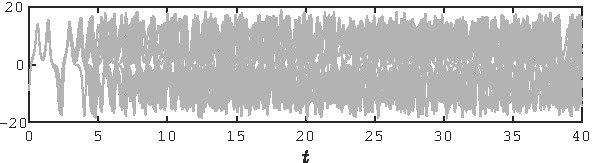
\includegraphics[scale=0.65]{LorenzTest1} \\
				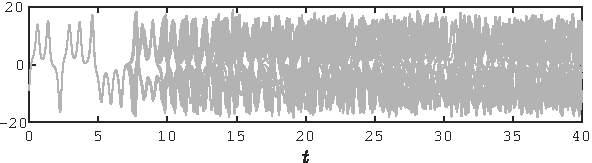
\includegraphics[scale=0.65]{LorenzTest2} \\
				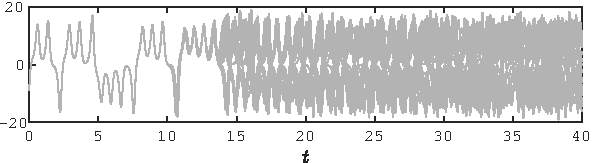
\includegraphics[scale=0.65]{LorenzTest3}
			\end{tabular}
		\end{center}
	\end{figure}	
	Solutions of the Lorenz system ($x$ component) -- {\color{BrickRed} different perturbations}
	\begin{center}
		{\color{ForestGreen} Which one has the correct magnitude wrt numerical error?}
	\end{center}
\end{frameT}

\begin{frameT}
	\frametitle{Motivation -- Error estimators}
	
	\begin{figure}
		\begin{center}
			\includegraphics[scale=0.9]{aPosteriori}
		\end{center}
	\end{figure}
	Error estimators for Lorenz given by \\
	{\color{BrickRed} Probabilistic solution:} use $\norm{\Var Y_n}^{1/2}$ where $Y_n$ is a probabilistic family\\
	{\color{NavyBlue} Classical embedded couple:} Local errors don't show the true behaviour!
	
	\vspace{0.5cm}
	{\color{ForestGreen} Goal:} A posteriori error estimator $\mathrm{err}_n \approx \norm{\Var Y_n}^{1/2}$ $\rightsquigarrow$ Work in progress!
\end{frameT}

\begin{frameT}
	\frametitle{Motivation -- Bayesian inverse problems}
	
	\begin{figure}
		\begin{center}
			
			\begin{tikzpicture}[scale=0.75, every node/.style={scale=0.75}]
			\draw (0,0) -- (9.2, 0) -- (9.2, 0.5) -- (0, 0.5) -- (0, 0);
			\draw[color=leg1,style=dotted,thick] (0.1, 0.25) -- (0.6, 0.25) node[right,color=black] {\small $\sigma=0.1$};
			\draw[color=leg2,style=dashdotted,thick] (2.1, 0.25) -- (2.6, 0.25) node[right,color=black] {\small$\sigma=0.05$};
			\draw[color=leg3,style=dashed,thick] (4.3, 0.25) -- (4.9, 0.25) node[right,color=black] {\small $\sigma=0.025$};			
			\draw[color=leg4,thick] (6.7, 0.25) -- (7.3, 0.25) node[right,color=black] {\small $\sigma=0.0125$};
			\end{tikzpicture}
			
			\vspace{0.2cm}
			\begin{tabular}{ccc}
				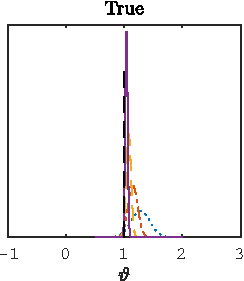
\includegraphics[scale=0.85]{ExPostTrue} & 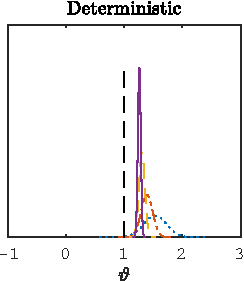
\includegraphics[scale=0.85]{ExPostRK} \includegraphics[scale=0.85]{ExPostRTS}
			\end{tabular}	
		\end{center}
	\end{figure}
	Posterior distributions (analytic) on $y_0$ for $y' = -y$, $y(0) = y_0$. One observation corrupted by noise $\mathcal N(0, \sigma^2)$ with truth $y_0^*$. \\
	For $\sigma \to 0$:
	\begin{itemize}
		\item {\color{ForestGreen} True solution:} Posterior converging to $\delta_{y_0^*}$ $\to$ good
		\item {\color{BrickRed} Runge-Kutta:} Posterior converging to Dirac delta on wrong value $\to$ bad
		\item {\color{NavyBlue} Probabilistic method:} Posterior variance $\approx$ numerical error
	\end{itemize}
\end{frameT}

%%%%%%%%%%%%%%%%%%%%%%%
% Geometric numerical integration
\section{Geometric numerical integration}

\begin{frame}
\frametitle{Notation}
Autonomous dynamical system, function $f\colon\R^d\to\R^d$ and the ODE
\begin{equation}
y' = f(y), \quad y(0) = y_0.
\end{equation}
{\color{ForestGreen} Flow} of the equation $\phi_t$
\begin{equation}
y(t) = {\color{ForestGreen}\phi_t(y_0)}.
\end{equation}
One-step method (e.g. Runge Kutta): {\color{NavyBlue} numerical flow} $\Psi_h$
\begin{equation}\label{eq:NumericalFlow}
y_{n+1} = {\color{NavyBlue}\Psi_h(y_n)}.
\end{equation}
\end{frame}

\begin{frameT}
	\frametitle{Geometric numerical integration}
	
	\begin{greenblock}[Goal]
		Develop numerical methods that preserve geometric properties of certain dynamical systems.
	\end{greenblock}
	
	\only<1>{{\color{NavyBlue}First integral} of motion $I \colon \R^d \to \R$
		\begin{equation}
		I(\phi_t(y_0)) = I(y_0), \quad \forall t > 0.
		\end{equation}
		{\color{ForestGreen} Example}: quadratic first integral, given $S \in \R^{d\times d}$, $v \in \R^d$
		\begin{equation}
		I(y) = y^\top S y + v^\top y,
		\end{equation}
		conserved by all Gauss collocation methods (e.g., {\color{NavyBlue} implicit midpoint}, ...).
		\begin{theorem}[Polynomial first integrals]
			No Runge-Kutta method can conserve all polynomial first integrals of degree $\mathrm{Deg}(I) \geq 3$.
		\end{theorem}
	}
	
	\only<2-3>{{\color{NavyBlue} Hamiltonian systems}: Given $Q \colon \R^{2d} \to \R$, define 
		\begin{equation}
		\begin{aligned}
		y'(t) &= J^{-1}\nabla Q(y), \quad &&y(0) = y_0 \\
		J &= \begin{pmatrix} 0 & I \\ -I & 0 \end{pmatrix}, \quad &&I \text{ identity in } \R^{d\times d}
		\end{aligned}
		\end{equation}
	}
	
	\only<2>{	
		The flow $\phi_t$ is {\color{ForestGreen} symplectic}
		\begin{equation}
		\phi_t'(y)^\top J \phi_t'(y) = J \implies \text{ Conservation of volumes }
		\end{equation}
		
		{\color{ForestGreen} Symplectic numerical methods}
		\begin{equation}
		\Psi_h'(y)^\top J \Psi_h'(y) = J
		\end{equation}
	}
	
	\only<3>{
		\begin{theorem} For a symplectic integrator of order $q$, there exist $C, \kappa >0$, independent of $h$ such that
		\begin{equation}
		\E \abs{Q(y_n) - Q(y_0)} \leq C_1 h^q,
		\end{equation}
		for time intervals of length $nh = \mathcal O(e^{\kappa/h})$. 
		\end{theorem}	
	}
	
\end{frameT}

\begin{frameT}
	\frametitle{Geometric numerical integration}
	
	\begin{greenblock}[Example] Two-body problem (planetary orbits), $y = (p, q)^\top \in \R^4$
		\begin{equation}
		Q(p, q) = \frac{1}{2}(p_1^2 + p_2^2) - \frac{1}{\sqrt{q_1^2 + q_2^2}}
		\end{equation}
	\end{greenblock}
	
	\only<1>{
		\begin{figure}
			\begin{tabular}{cc}
				\includegraphics[]{KeplerEE} & \includegraphics[]{KeplerSE}
			\end{tabular}
		\end{figure}
	}	
	
	\only<2>{
		\begin{figure}
			\centering
			\includegraphics[]{KeplerEnergy}
		\end{figure}
	}
\end{frameT}

\begin{frameT}
	\frametitle{Geometric numerical integration}
	
	\only<1>{Given Hamiltonian $Q(p, q)$.}
	\only<2>{Given {\color{NavyBlue} separable} Hamiltonian $Q(p, q) = Q_1(p) + Q_2(q)$.}
	
	\only<1>{\begin{greenblock}[Symplectic Euler method -- order 1]
			\begin{equation}
			\begin{aligned}
			p_{n+1} &= p_n - h Q_q(p_{n+1}, q_n),\\
			q_{n+1} &= q_n + h Q_p(p_{n+1}, q_n).
			\end{aligned}
			\end{equation}
		\end{greenblock}
		
		\begin{greenblock}[Störmer-Verlet scheme -- order 2]
			\begin{equation}
			\begin{aligned}
			p_{n+1/2} &= p_n - \frac{h}{2} Q_q(p_{n+1/2}, q_n),\\
			q_{n+1} &= q_n + \frac{h}{2} \big(Q_p(p_{n+1/2}, q_n) + Q_p(p_{n+1/2}, q_{n+1})\big), \\
			p_{n+1} &= p_n - \frac{h}{2} Q_q(p_{n+1/2}, q_{n+1}).
			\end{aligned}
			\end{equation}
	\end{greenblock}}
	
	\only<2>{
		\begin{greenblock}[Symplectic Euler method -- order 1, explicit]
			\begin{equation}
			\begin{aligned}
			p_{n+1} &= p_n - h Q_2'(q_n),\\
			q_{n+1} &= q_n + h Q_1'(p_{n+1}).
			\end{aligned}
			\end{equation}
		\end{greenblock}
		
		\begin{greenblock}[Störmer-Verlet scheme -- order 2, explicit]
			\begin{equation}
			\begin{aligned}
			p_{n+1/2} &= p_n - \frac{h}{2} Q_2'(q_n),\\
			q_{n+1} &= q_n + h Q_1'(p_{n+1/2}), \\
			p_{n+1} &= p_n - \frac{h}{2} Q_2'(q_{n+1}).
			\end{aligned}
			\end{equation}
		\end{greenblock}
		
		Several examples of separable Hamiltonians ({\color{NavyBlue} Two-body problem, ...})
		
	}
	
\end{frameT}

%%%%%%%%%%%%%%%%%%%%%%%
% Probabilistic methods for ODEs
\section{Probabilistic methods for ODEs}

\begin{frame}
\frametitle{Probabilistic methods for ODEs}

{\color{ForestGreen} Filtering} methods for ODEs: fix a prior on $y(t)$ (Gaussian process), update with evaluations of $f(y)$.
	\begin{itemize}
		\item \cite{KeH16, KSH18}
		\item \cite{CCC16}
		\item \cite{SDH14, SSH18}
		\item \ldots
	\end{itemize}

\vspace{0.5cm}
{\color{NavyBlue} Randomised} methods for ODEs: random perturbation of deterministic numerical solutions $\to$ sampling
\begin{itemize}
	\item \cite{CGS16}
	\item \cite{LSS17}
	\item \cite{AbG18}
	\item \ldots
\end{itemize}
\end{frame}

\begin{frameT}
\frametitle{Additive noise method}

Stochastic process $\{Y_n\}_{n=1, 2, \ldots}$ with recurrence
\begin{equation}
Y_{n+1} = \underbrace{\Psi_h(Y_n)}_{\text{{\color{ForestGreen} deterministic}}} + \underbrace{\xi_n(h)}_{\text{{\color{NavyBlue} random}}}.
\end{equation}
{\color{BrickRed} Main assumption}: For $p > 1$ and $Q \in \R^{d\times d}$
\begin{equation}
	\xi_n(h) \iid \mathcal N(0, Qh^{2p+1}).
\end{equation}

\only<2>{
\begin{greenblock}[Properties]
	If $\Psi_h$ is of order $q$ and for $\Phi\colon\R^d\to\R$ smooth
	\begin{itemize}
		\item Strong convergence: $\E\norm{y(hn)-Y_n} \leq Ch^{\min\{p, q\}}$,
		\item Weak convergence: $\abs{\Phi\big(y(hn)\big) - \E\Phi(Y_n)} \leq Ch^{\min\{2p, q\}}$,
		\item Good qualitative behavior in Bayesian inverse problems.
	\end{itemize}
\end{greenblock}
}

\only<3>{
\begin{redblock}[Issues]
	\begin{itemize}
		\item Robustness: $\Psi_h(Y_{n-1}) > 0 \centernot\implies \Pr(Y_n < 0) = 0$,
		\item Geometric properties are not conserved from $\Psi_h$.
	\end{itemize}
\end{redblock}
}
\end{frameT}

\begin{frameT}
\frametitle{Random time steps}

{\color{ForestGreen}Intrinsic noise}: Random time-stepping Runge-Kutta (RTS-RK)
\begin{equation}
Y_{n+1} = \Psi_{{\color{NavyBlue} H_n}}(Y_n),
\end{equation}
{\color{BrickRed}Main assumption}: $\{H_n\}_{n=0,1,\ldots}$ iid such that for $h, C > 0$ and $p > 1$
\begin{equation}
H_n > 0 \text{ a.s.}, \quad \E H_n = h, \quad \Var H_n = Ch^{2p + 1}.
\end{equation} 
Example: $H_n \iid \mathcal{U}(h-h^{p+1/2}, h+h^{p+1/2})$.

\only<2>{
\begin{greenblock}[Properties]
	If $\Psi_h$ is of order $q$ and for $\Phi\colon\R^d\to\R$ smooth
	\begin{itemize}
		\item Strong convergence: $\E\norm{y(hn)-Y_n} \leq Ch^{\min\{p, q\}}$,
		\item Weak convergence: $\abs{\Phi\big(y(hn)\big) - \E\Phi(Y_n)} \leq Ch^{\min\{2p, q\}}$,
		\item Good qualitative behavior in Bayesian inverse problems.
	\end{itemize}
\end{greenblock}
}

\only<3>{
\begin{greenblock}[Properties -- Geometric]
	\begin{itemize}
		\item Conservation of (polynomial) first integrals is inherited by $\Psi_h$,
		\item Flow map is symplectic if $\Psi_h$ is symplectic, 
		\item Long-time conservation of energy in Hamiltonian systems. 
	\end{itemize}
\end{greenblock}
}
\end{frameT}

\begin{frame}
\frametitle{Conservation of first integrals -- Additive noise}

{\color{BrickRed} Recall}: $Y_{n+1} = \Psi_h(Y_n) + \xi_n(h)$, with $\E\xi_n(h) \xi_n(h)^\top = h^{2p+1}Q$

\vspace{0.4cm}	
{\color{ForestGreen} Linear first integrals}: $I(y) = v^\top y$ such that $I(\Psi_h(Y_1)) = I(y_0)$. Then
\begin{equation}
I(Y_1) = v^\top  (y_0 + \xi_0(h)) \implies \E I(Y_1) = I(y_0) \text{ iff } \E \xi_0(h) = 0.
\end{equation}

\vspace{0.4cm}
{\color{NavyBlue} Quadratic first integrals}: $I(y) = y^\top S y$ such that $I(\Psi_h(Y_1)) = I(y_0)$. Then
\begin{equation}
\begin{aligned}
&I(Y_1) = I(y_0) + 2\xi_0(h)^T S  \Psi_h(y_0) + \xi_0(h)^T S \xi_0(h), \\
&\implies \E I(Y_1) = I(y_0) + {\color{BrickRed}Q : S h^{2p + 1}}, \quad (\text{with } \E \xi_0(h) = 0)
\end{aligned}
\end{equation}
Quadratic first integrals are not conserved on average! 

\end{frame}

\begin{frame}
\frametitle{Conservation of first integrals}

\begin{theorem}[Conservation of invariants] If the Runge-Kutta scheme defined by $\Psi_h$ conserves an invariant $I(y)$ for an ODE, then the RTS-RK method conserves $I(y)$ for the same ODE.
\end{theorem}

\vspace{0.2cm}
{\color{NavyBlue} Proof}\\
If $I(\Psi_h(y)) = I(y)$ for any $h$, then $I(\Psi_{H_0}(y)) = I(y)$ for any value that $H_0$ can assume.
\end{frame}

\begin{frameT}
	\frametitle{Symplecticity}
	
	Energy $Q \colon \R^{2d} \to \R$ and Hamiltonian system
	\begin{equation}
	y' = J^{-1} \nabla Q(y), \quad J = \begin{pmatrix} 0 & I \\ -I & 0 \end{pmatrix}.
	\end{equation}
	Symplectic integrator $\Psi_h$ of order $q$.
	
	\begin{theorem}[Strong approximation of the Hamiltonian] There exist positive constants $\kappa, C_1, C_2, C_3$, independent of $h$ such that
		\begin{equation}
		\E \abs{Q(Y_n) - Q(y_0)} \leq C_1 h^q,
		\end{equation}
		for time intervals of length $\mathcal O(h^{1-2p})$. 
	\end{theorem}
	
	\only<2>{
		{\color{NavyBlue} Idea of the proof} \\
		Use classical backward error analysis. Considering that $\E H_k = h$, we have at ``first order'' the same conservation as deterministic methods. The time interval reduction comes from the time steps' variance.
	}

\end{frameT}

\begin{frame}
\frametitle{Numerical experiments -- Geometric properties}
Consider the perturbed Kepler equation (model for two-body problem)
\begin{equation}
\begin{aligned}
w_1' &= v_1, && v_1' = -\frac{w_1}{\norm{w}^3} {\color{BrickRed}- \frac{\delta w_1}{\norm{w}^5}}, \\
w_2' &= v_2, && v_2' = -\frac{w_2}{\norm{w}^3} {\color{BrickRed}- \frac{\delta w_2}{\norm{w}^5}}.
\end{aligned}
\end{equation}
The {\color{NavyBlue} angular momentum} is conserved (quadratic first integral)
\begin{equation}
I(v, w) = w_1v_2 - w_2v_1
\end{equation}
$\to$ employ a Gauss method (implicit midpoint rule).

\end{frame}

\begin{frameT}
\frametitle{Numerical experiments -- Geometric properties}
\only<1>{
\begin{figure}
\begin{center}
	\begin{tabular}{c@{\hspace{0.3cm}}c}
		\includegraphics[width=0.2\linewidth]{KeplerOne} & \includegraphics[width=0.2\linewidth]{KeplerTwo} \\
		\includegraphics[width=0.2\linewidth]{KeplerOneAdd} & \includegraphics[width=0.2\linewidth]{KeplerTwoAdd} \\
	\end{tabular}
\end{center}
\end{figure}
{\color{NavyBlue} RTS-RK} (first row), {\color{ForestGreen} Additive noise} (second row). Time $0 \leq t \leq 200$ and $200 \leq t \leq 400$ (left and right)
}
\only<2>{
\begin{figure}
\hspace{-0.5cm}\includegraphics[width=0.8\linewidth]{KeplerMom}
\end{figure}
Conservation of the {\color{NavyBlue} angular momentum} (quadratic first integral)
}
\end{frameT}

\begin{frameT}
\frametitle{Numerical experiments -- Geometric properties}
Consider the pendulum system, Hamiltonian with {\color{NavyBlue} energy}
\begin{equation}
Q(v, w) = \frac{1}{2}v^2 - \cos(w).
\end{equation}
Energy is separable: $Q(v, w) = Q_1(v) + Q_2(w)$.

\only<1>{
\begin{greenblock}[Störmer-Verlet scheme -- order 2]
	\begin{equation}
	\begin{aligned}
		v_{n+1/2} &= v_n - \frac{h}{2} Q_w(v_{n+1/2}, w_n),\\
		w_{n+1} &= w_n + \frac{h}{2} \big(Q_v(v_{n+1/2}, w_n) + Q_v(v_{n+1/2}, w_{n+1})\big), \\
		v_{n+1} &= v_n - \frac{h}{2} Q_w(v_{n+1/2}, w_{n+1}).
	\end{aligned}
	\end{equation}
\end{greenblock}}

\only<2>{
\begin{greenblock}[Störmer-Verlet scheme -- order 2, explicit]
	\begin{equation}
	\begin{aligned}
	v_{n+1/2} &= v_n - \frac{h}{2} Q_2'(w_n),\\
	w_{n+1} &= w_n + h Q_1'(v_{n+1/2}), \\
	v_{n+1} &= v_n - \frac{h}{2} Q_2'(w_{n+1}).
	\end{aligned}
	\end{equation}
\end{greenblock}}

\end{frameT}

\begin{frame}
\frametitle{Numerical experiments -- Geometric properties}

\begin{figure}
\includegraphics[width=0.5\linewidth]{MeanTime}
\end{figure}

Mean error on the Hamiltonian for different values of the time step $h$.

\end{frame}

\section{Bayesian inverse problems}

\begin{frameT}
\frametitle{Bayesian inverse problems}

\begin{greenblock}[Goal] Given $\theta \in \R^n$, $f_\theta \colon \R^d \to \R^d$ and the ODE
\begin{equation}
y' = f_\theta(y), \quad y(0) = y_{0, \theta} \in \R^d,
\end{equation}
retrieve the true value $\theta^*$ from observations of $y(t)$, $t > 0$.		
\end{greenblock}

\only<2> {
\vspace{0.2cm}
{\color{BrickRed} Bayesian setting}: fix prior $\pi_{\mathrm{prior}}(\theta)$, consider the forward operator $\mathcal{G}$ and model observations as
\begin{equation}
\underbrace{\vphantom{\mathcal{G}(\theta^*)} \mathcal{Y}}_{ {\color{BrickRed} \text{observations}}} = 
\underbrace{\mathcal{G}(\theta^*)}_{{\color{ForestGreen}\text{forward}}} + 
\underbrace{\vphantom{\mathcal{G}(\theta^*)} \epl}_{{\color{NavyBlue}\text{noise}}}, 
\quad \epl \sim \pi_{\mathrm{noise}},
\end{equation} 	
then the {\color{BrickRed} posterior distribution (density)} is
\begin{equation}
\pi(\theta \mid \mathcal{Y}) \propto \pi_{\mathrm{prior}}(\theta) \pi_{\mathrm{noise}}(\mathcal{Y} - \mathcal{G}(\theta)).
\end{equation}
}
\end{frameT}

\begin{frameT}
\frametitle{Bayesian inverse problems}

\vspace{1cm}
\only<1-2>{
The posterior $\pi(\theta \mid \mathcal{Y})$ is not computable, approximate with
\begin{equation}
{\color{ForestGreen}\pi^h}(\theta \mid \mathcal{Y}) \propto \pi_{\mathrm{prior}}(\theta) \pi_{\mathrm{noise}}(\mathcal{Y} - {\color{ForestGreen}\mathcal{G}^h}(\theta)).
\end{equation}
}
\only<3-4>{
The posterior $\pi(\theta \mid \mathcal{Y})$ is not computable, approximate with
\begin{equation}
{\color{NavyBlue}\pi^{h, \mathrm{RTS}}}(\theta \mid \mathcal{Y}) \propto \pi_{\mathrm{prior}}(\theta) {\color{NavyBlue}\E^{\mathbf{H}}}\pi_{\mathrm{noise}}(\mathcal{Y} - {\color{NavyBlue}\mathcal{G}^{\mathbf{H}}}(\theta)),
\end{equation}
where $\mathbf{H} = (H_0, H_1, \ldots)$ is the vector of all time steps chosen in one run.
}
\only<2>{
\begin{greenblock}[Properties]
$\pi^h \to \pi$ for $h \to 0$ (in the Hellinger distance).
\end{greenblock}
\begin{redblock}[Issue]
\begin{itemize}
	\item $\pi^h$ concentrated around values ``far'' from $\theta^{*}$ $\to$ non-predictive posterior
\end{itemize}
\end{redblock}
}
\only<4>{
\begin{greenblock}[Properties]
\begin{itemize}
	\item $\pi^{h, \mathrm{RTS}} \to \pi$ for $h \to 0$ (in the Hellinger distance). \cite{LST17}
	\item ``correct'' the non-predictive behaviour of deterministic approximations
\end{itemize}
\end{greenblock}
\begin{orangeblock}[Warning]
\begin{itemize}
	\item Approximation of $\E^{\mathbf{H}}\pi_{\mathrm{noise}}(\mathcal{Y} - \mathcal{G}^{\mathbf{H}}(\theta))$ is required
\end{itemize}
\end{orangeblock}
}	
\end{frameT}

\begin{frame}
\frametitle{Numerical experiment -- Bayesian inverse problems}
Consider the Hénon-Heiles system (motion of a star around a galactic center), Hamiltonian with {\color{NavyBlue} energy}
\begin{equation}\label{eq:HamHH}
E(v, w) = \frac{1}{2}\norm{v}^2 + \frac{1}{2}\norm{w}^2 + w_1^2w_2 - \frac{1}{3}w_2^3.
\end{equation}
Chaotic problem for certain levels of energy.
\begin{greenblock}[Goal]
Find posterior $\pi((v_0, w_0) \mid \mathcal{Y})$ over the initial condition from a single observation of $(v(10), w(10))$ 
\end{greenblock}
\end{frame}

\begin{frame}
\frametitle{Numerical experiment -- Bayesian inverse problems}
\only<1>{
\begin{figure}
\begin{center}
\begin{tabular}{c@{\hspace{0.3cm}}c}
\includegraphics[width=0.4\linewidth]{BayesHeun} & \includegraphics[width=0.4\linewidth]{BayesHeun2} \\ 
\end{tabular}
\end{center}
\end{figure}
Posterior distributions given by {\color{BrickRed} deterministic Heun method}.}

\only<2>{
\begin{figure}
\begin{center}
\begin{tabular}{c@{\hspace{0.3cm}}c}
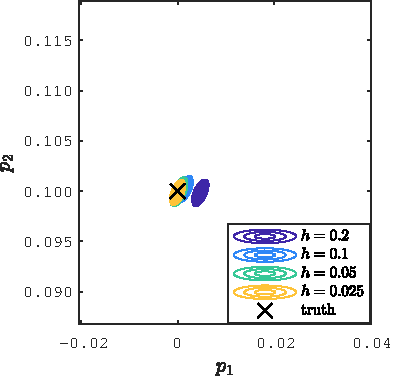
\includegraphics[width=0.4\linewidth]{BayesDet} & \includegraphics[width=0.4\linewidth]{BayesDet2} \\ 
\end{tabular}
\end{center}
\end{figure}
Posterior distributions given by {\color{NavyBlue} deterministic Störmer-Verlet method}.}

\only<3>{
\begin{figure}
\begin{center}
\begin{tabular}{c@{\hspace{0.3cm}}c}
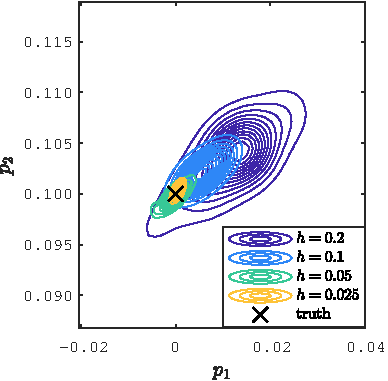
\includegraphics[width=0.4\linewidth]{BayesProb} & \includegraphics[width=0.4\linewidth]{BayesProb2} \\ 
\end{tabular}
\end{center}
\end{figure}
Posterior distributions given by {\color{ForestGreen} RTS-RK Störmer-Verlet method}.}
\end{frame}

\appendix
\begin{frame}
\frametitle{References}

\setbeamertemplate{bibliography item}[text]

\scriptsize{
\begin{thebibliography}{10}
\bibitem[Abdulle and Garegnani, 2018]{AbG18}
A. Abdulle, G. Garegnani (2018).
\newblock Random time step probabilistic methods for uncertainty quantification in chaotic and geometric numerical integration.
\newblock {\em preprint arXiv:1801.01340}

\bibitem[Chkrebtii et~al., 2016]{CCC16}
O.~A. Chkrebtii, D.~A. Campbell, B.~Calderhead, M.~A. Girolami (2016).
\newblock Bayesian solution uncertainty quantification for differential	equations.
\newblock {\em Bayesian Anal.}

\bibitem[Conrad et~al., 2016]{CGS16}
Conrad, P.~R., Girolami, M., S{\"a}rkk{\"a}, S., Stuart, A., and Zygalakis, K.
(2016).
\newblock Statistical analysis of differential equations: introducing
probability measures on numerical solutions.
\newblock {\em Stat. Comput.}

\bibitem[Kersting and Hennig, 2016]{KeH16}
Kersting, H., Hennig, P. (2016).
\newblock Active uncertainty calibration in {B}ayesian {ODE} solvers.
\newblock In {\em Proceedings of the 32nd Conference on Uncertainty in Artificial Intelligence (UAI 2016)}, pages 309--318. {AUAI} Press.

\bibitem[Kersting et~al., 2018]{KSH18}
Kersting, H., Sullivan, T.~J., and Hennig, P. (2018).
\newblock Convergence rates of {G}aussian {ODE} filters.
\newblock {\em preprint arXiv:1807.09737}

\bibitem[Lie et~al., 2017]{LSS17}
Lie, H.~C., Sullivan, T.~J., and Stuart, A. (2017).
\newblock Strong convergence rates of probabilistic integrators for ordinary differential equations.
\newblock {\em preprint arXiv:1703.03680}

\bibitem[Lie et~al., 2017]{LST17}
Lie, H.~C., Sullivan, T.~J., and Teckentrup, A.~L. (2017).
\newblock Random forward models and log-likelihoods in Bayesian inverse	problems.
\newblock {\em preprint arXiv:1712.05717}

\bibitem[Schober et~al., 2014]{SDH14}
Schober, M, Duvenaud, D. and Hennig, P. (2014).
\newblock Probabilistic ODE solvers with Runge-Kutta means.
\newblock {\em preprint arXiv:1406.2582}

\bibitem[Schober et~al., 2018]{SSH18}
Schober, M, S{\"a}rkk{\"a}, S. and Hennig, P. (2014).
\newblock A probabilistic model for the numerical solution of initial value problems.
\newblock {\em Stat. Comput.}

\end{thebibliography}
}

\end{frame}

\end{document}
